% LATEX TEMPLATE 
% adapted from https://infinitedescent.xyz/latex/ by wade_

\documentclass[11pt]{article}

% Edit the following to change the title, author name and date
\title{Calc in 3d Notes}
\author{saffron\_}
\date{}

% Packages
\usepackage{amsmath}
\usepackage{amsfonts}
\usepackage{amssymb}
\usepackage{amsthm}
\usepackage{enumerate}
\usepackage{geometry}
\usepackage{graphicx}
\usepackage{hyperref}
\usepackage{multicol}
% \usepackage[colorlinks=true,linkcolor=magenta]{hyperref}

% Page setup
\setlength{\parskip}{10pt}
\setlength{\parindent}{0pt}
\geometry{
    paper={letterpaper}, % Change to 'a4paper' for A4 size
    marginratio={1:1},
    margin={1in}
}

% Theorem environments
\theoremstyle{definition}
\newtheorem{theorem}{Theorem}
\newtheorem{lemma}[theorem]{Lemma}
\newtheorem{corollary}[theorem]{Corollary}
\newtheorem{proposition}[theorem]{Proposition}
\newtheorem{definition}[theorem]{Definition}
\newtheorem{example}[theorem]{Example}

% Custom per each document
\newcommand{\addsection}[1]{\section*{#1}\addcontentsline{toc}{section}{#1}} % for adding \section*{} sections to \tableofcontents
\newcommand{\bb}[1]{\mathbb{#1}} % love of my life
% \newcommand{\floor}[1]{\left\lfloor #1 \right\rfloor}
% \newcommand{\ceil}[1]{\left\lceil #1 \right\rceil}
\newcommand{\col}[1]{\begin{minipage}{\columnwidth}#1\end{minipage}}
\newcommand{\magn}[1]{\left\lVert #1 \right\rVert}
\DeclareMathOperator{\proj}{proj}
\DeclareMathOperator{\comp}{comp}

\graphicspath{ {./media/} }

\begin{document}
\maketitle
\tableofcontents

%%%%%%%%%%%%%%%%%%%%%%%%%%%%
%% Start of document body %%
%%%%%%%%%%%%%%%%%%%%%%%%%%%%

\newpage
\addsection{Chapter 2: Vectors in Space}

\begin{multicols}{2}[Graphing]
  \col{
    \centering
    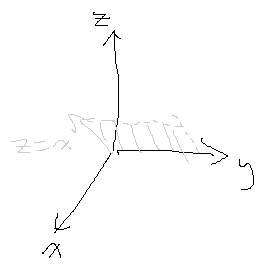
\includegraphics{3d_space.png}
    \emph{convention}
  }
  \col{
    \centering
    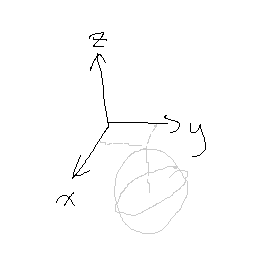
\includegraphics{sphere.png}
    \emph{sphere:} $(x-1)^2 + (y-2)^2 + (z+3)^2 = 9$
  }
\end{multicols}

\begin{multicols}{2}[The Vector]
  \col{
    \centering
    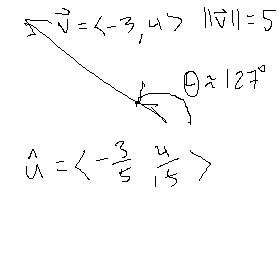
\includegraphics{vector.png}
  }
  \col{
    \begin{itemize}
      \item a quantity with a magnitude and direction
      \item unit vector $\displaystyle\hat{u} =\frac{\vec{v}}{\lVert \vec{v} \rVert}$
    \end{itemize}
  }
\end{multicols}

\newpage
\begin{multicols}{3}[Vector Operations]
  \col{
    \begin{itemize}
      \item Addition
      \begin{itemize}
        \item $\vec{a} = \left< 1,2 \right>$,  $\vec{b} = \left< 3,4 \right>$
        \item $\vec{a} + \vec{b} = \left< 4,6 \right>$
      \end{itemize}
    \end{itemize}
  }
  \col{
    \begin{itemize}
      \item Scalar Multiplication
      \begin{itemize}
        \item $\vec{v} = \left< 1,3 \right>$, $c = 2$
        \item $c\vec{v} = \left< 2,6 \right>$
      \end{itemize}
    \end{itemize}
  }
  \col{
    simple inverses for subtraction and scalar division exist.
  }
\end{multicols}
\begin{multicols}{2}
  \col{
    \begin{itemize}
      \item Dot Product (also 2d!)
      \begin{itemize}
        \item geom.:
        
        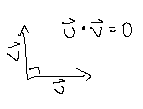
\includegraphics{dot_prod.png} \\
        $\vec{u} \cdot \vec{v} = \magn{\vec{u}} \magn{\vec{v}}\cos \theta$
        \item alg.:
        
        $\vec{u} = \left< u_1, u_2, u_3 \right>$, 
        $\vec{v} = \left< v_1, v_2, v_3 \right>$\\
        $\vec{u} \cdot \vec{v} = \sum u_i v_i$
        \item $\vec{v}\cdot\vec{v} = \magn{\vec{v}}^2$
        \item two vectors are orthogonal aka $\perp$ iff their dot product is $0$
        \item $\displaystyle\cos \theta = \frac{\vec{u} \cdot \vec{v}}{\magn{u}\magn{v}}$ wtf is equation 2.5 "unique over this range" on abt
        \item work $= \vec{F} \cdot \vec{D}$
        \item $\comp$ (scalar projection)
        \begin{align*}
          \comp_{\vec{u}} \vec{v} & = \magn{\vec{v}} \cos \theta \\
          & = \frac{\vec{u} \cdot \vec{v}}{\magn{\vec{u}}}
        \end{align*}
        \item $\proj$ (vector projection)
        \begin{align*}
          \proj_{\vec{u}} \vec{v} &= \comp_{\vec{u}} \vec{v} \cdot \frac{\vec{u}}{\magn{\vec{u}}} \\
          &= \frac{\vec{u}\cdot\vec{v}}{\magn{\vec{u}}^2}\vec{u}
        \end{align*}
      \end{itemize}
    \end{itemize}
  }
  \col{
    \begin{itemize}
      \item Cross Product (3d)
      \begin{itemize}
        \item geom.:
        
        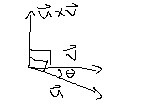
\includegraphics{cross_prod.png}\\
        $\magn{\vec{u}\times\vec{v}} = \magn{\vec{{u}}}\magn{\vec{v}}\sin\theta$
        \item alg.:
        \item $\vec{u} \times \vec{v} = \det\begin{vmatrix}
          \hat{\imath} & \hat{\jmath} & \hat{k}\\
          u_1 & u_2 & u_3 \\
          v_1 & v_2 & v_3
        \end{vmatrix}$
        \item result is $\perp$ to both input vectors, \\
        direction by right hand rule
        \item triple scalar product: \\
        $\vec{u} \cdot (\vec{v}\times\vec{w}) \\ 
        = (\vec{u}\times\vec{v})\cdot\vec{w} \\
        = \det\begin{vmatrix}
          u_1 & u_2 & u_3 \\
          v_1 & v_2 & v_3 \\
          w_1 & w_2 & w_3
        \end{vmatrix}$
        \item if $\vec{u}$ and $\vec{v}$ are the sides of a parallelogram, then its area is $\magn{\vec{u}\times\vec{v}}$
        \item if a parallelepiped has edges $\vec{u}, \vec{v}, \vec{w}$, its volume is the absolute value of its triple scalar product
        \item torque $= \vec{\tau} = \vec{r} \times \vec{F}$
      \end{itemize}
    \end{itemize}
  }
\end{multicols}

\newpage
\begin{multicols}{2}
  \col{
    Lines
    \begin{enumerate}[(1)]
      \item Vector Equation Form
      
      $\vec{r} = \vec{r_0} + t\vec{v}$ \\
      eg $\left<x,y,z\right> = \left<1,2,-5\right> + t\left<3,-4,-1\right>$
      \item Parametric Equation Form
      \begin{align*}
        x &= 1+3t \\
        y &= 2-4t \\
        z &= -5-t 
      \end{align*}
      
      \item Symmetric Equation Form 
      
      solve for $t$
      \[\frac{x-1}{3} = \frac{y-2}{-4} = \frac{z+5}{-1}\]

      \item Edge Case: 0-component
      
      Let a line be defined by the point and vector $(1,-2,6)$ and $\left<3,7,0\right>$. We say the line is:
      \[ \frac{x-1}{3} = \frac{y+2}{7}, z=6 \]
    \end{enumerate}
    \begin{itemize}
      \item point to line distance: use paralleogram area trick
    \end{itemize}

    Planes
    \begin{enumerate}[(1)]
      \item Vector Equation Form
      
      $(\vec{r}-\vec{r_0})\cdot \vec{n} = 0$ \\
      eg $(\left<x,y,z\right>-\left<1,0,1\right>) \cdot \left<1,2,-3\right> = 0$
      \item Scalar Equation, "General" Form
      
      $ax +by +cz +d = 0$
    \end{enumerate}
    \begin{itemize}
      \item point to plane distance: use $\comp_{\vec{u}}\vec{v}$ trick
      \item angle between planes: same as angle between their normal vectors
    \end{itemize}

    Quadric Surfaces
    \begin{itemize}
      \item cylinder: 3d shape consisting of all parallel lines (eg $y=3x^2$)
      \item see \url{quadric_surfaces.pdf}
    \end{itemize}
  }
  \col{
    \addsection{Chapter 3: Vector-Valued Functions}
    Vector-Valued Function
    $${\vec{r}(t) = \left<f(t), g(t), h(t)\right>}, i < t < j$$

    Unit Circle Parameterization
    
    temp\\

    Limits of VVFs
    \begin{itemize}
      \item pass them into the vec. pretty intuitive
      \item a VVF $\vec{r}(a)$ is cont. at $a$ iff $\displaystyle\lim_{t\rightarrow a}\vec{r}(t) = \vec{r}(a)$ (and both are defined )
    \end{itemize}

    Calc with VVFs
    \begin{itemize}
      \item derivatives are intuitive. use the corresponding dot/cross/scalar in deriving $\vec{u}\cdot\vec{v}$
      \item unit tangent vector is the derivative's unit vector
      \item integrals are intuitive. consider constant vector $C$ instead of scalar constant
    \end{itemize}

    Consult exam 1 cheatsheet for notes on the rest of the chapter
  }
\end{multicols}

\newpage
\addsection{Chapter 4: Differentiation}
\begin{multicols}{2}
  \col{
    Functions of Multiple Variables
    \begin{itemize}
      \item domain: analyze what values are invalid
      \item range: image of domain
      \item level planes/level surfaces/contour maps: setting the function to some constant and drawing out the resulting shape 
    \end{itemize}

    Limits and Continuity
    \begin{itemize}
      \item limit rules are identical to 2d, including
      \item limits must be unique. ie, the $\delta$ disk around a point must only contain one value. (disprove limit by finding different values through different ``paths'' to the limit)
      \item as in 2d, $f(x,y)$ is continuous at $(a,b)$ iff
      \[  \lim_{(x,y)\rightarrow(a,b)}f(x,y) = f(a,b)\]
      with both defined.
      \item sum, product, comp of cont functions: cont
    \end{itemize}

    Partial Derivatives
    \begin{itemize}
      \item slope of line in a direction, at a point
      \item Limit definition:
      \[ \frac{\partial f}{\partial x} = \lim_{h\rightarrow 0}\frac{f(x+h,y)-f(x,y)}{h}\]
      \item four second order partials exist
      \begin{gather*}
        \frac{\partial^2 f}{\partial x^2} = \frac{\partial}{\partial x}\left[\frac{\partial f}{\partial x}\right] = f_{xx} \\
        \frac{\partial^2 f}{\partial x\partial y} = \frac{\partial}{\partial x}\left[\frac{\partial f}{\partial y}\right] = f_{yx} \\
        \frac{\partial^2 f}{\partial y\partial x} = \frac{\partial}{\partial y}\left[\frac{\partial f}{\partial x}\right] = f_{xy} \\
        \frac{\partial^2 f}{\partial y^2} = \frac{\partial}{\partial y}\left[\frac{\partial f}{\partial y}\right] = f_{yy} \\
      \end{gather*}
      \item Clairaut's Thrm: if $f_{xy}$ and $f_{yx}$ are cont near a point, they are equal
    \end{itemize}
  }
  \col{
    Tangent Planes
    \begin{itemize}
      \item if all tangent lines to a point are in the same plane, call that the tangent plane
      \begin{itemize}
        \item (not true if there is a point)
        \item maybe theres a correlation somewhere with differentiability? (p393)
      \end{itemize}
      \item the tangent plane to $z = f(x,y)$ at $(a,b)$ is 
      \[ z = f(a,b) + f_x(a,b)(x-a) + f_y(a,b)(y-b) \]
      \item find an approx at $(a,b)$ via the linear approximation plane $L(x,y) = $ RHS (above)
      \item a function is differentiable at $(a,b)$ iff
      \[ f(x,y) = \text{RHS} + E(x,y) \]
      where the error term $E$ satisfies
      \[ \lim_{(x,y)\rightarrow(a,b)}\frac{E(x,y)}{\sqrt{(x-a)^2+(y-b)^2}} = 0. \]
      alternatively, if $f$, $f_x$, and $f_y$ exist near $(a,b)$ and are cont. at $(a,b)$, then $f$ is differentiable there.
      \item let $z=f(x,y)$ with $(a,b)$ in the domain of $f$, and let $\Delta x$ and $\Delta y$ be chosen such that $(a+\Delta x,b+\Delta y)$ is also in the domain of $f$.
      
      then
      \begin{gather*}
        dx = \Delta x \\
        dy = \Delta y \\
        dz = f_x(a,b)dx + f_y(a,b)dy.
      \end{gather*}
      $dx$ and $dy$ are differentials, $dz$ the ``total differential,'' and we estimate error with it.

      notice the similarity to the tangent plane equation.
    \end{itemize}
  }
\end{multicols}

\begin{multicols}{2}
  \col{
    The Chain Rule
    \begin{itemize}
      \item consider
      \begin{gather*}
        w=f(x,y,z) \\
        x = x(t,u,v) \\
        y = y(t,u,v) \\
        z = z(t,u,v) \\
        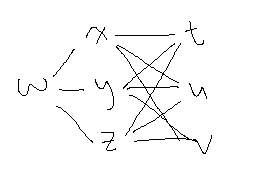
\includegraphics{chain_rule_treediagram.png}.
      \end{gather*}
      then,
      \begin{gather*}
        \frac{\partial w}{\partial t} = 
          \frac{\partial w}{\partial w}\frac{\partial x}{\partial t}
          + \frac{\partial w}{\partial y}\frac{\partial y}{\partial t}
          + \frac{\partial w}{\partial z}\frac{\partial z}{\partial t}.
      \end{gather*}
      others are left as an exercise to the reader.
    \end{itemize}

    Implicit Differentiation
    \begin{itemize}
      \item consider $x^2 + 3y^2 + 4y - 4 = 0$. 
      
      to find $\frac{dy}{dx}$, we may implicitly differentiate this by taking $\frac{d}{dx}$ of both sides and solving.

      but we may also define 
      \[ f(x,y) = x^2 + 3y^2 + 4y - 4, f(x,y) = 0.\]
      with this in mind, suppose $f(x,y)=0$. then,
      \[ \frac{dy}{dx} = -\frac{\partial f/\partial x}{\partial f/\partial y} \]
      and if $f(x,y,z) = 0$,
      \[ \frac{\partial z}{\partial x} = -\frac{\partial f/\partial x}{\partial f/\partial z}, \frac{\partial z}{\partial y} = -\frac{\partial f/\partial y}{\partial f/\partial z}.\]
      these can be derived from the chain rule.
    \end{itemize}
  }
  \col{
    Directional Derivatives and the Gradient
    \begin{itemize}
      \item the directional derivative of $f(x,y)$ in the direction $\hat{u} = \left<\cos\theta, \sin\theta\right>$ is
      \[ D_{\hat{u}}f(a,b) = \lim_{h\rightarrow 0}\frac{f(a+h\cos\theta, b+h\sin\theta)-f(a,b)}{h}\]
      alternatively, if the partials exist,
      \begin{align*}
        D_{\hat{u}}f(x,y) &= f_x(x,y)\cos\theta + f_y(x,y)\sin\theta \\
        &= \left<\,f_x(x,y), f_y(x,y)\,\right> \cdot \hat{u} \\
        % &= [\,f_x(x,y)\hat{\i} + f_y(x,y)\hat{\j}\,] \cdot \hat{u} \\
        &= \nabla f(x,y) \cdot \hat{u}.
      \end{align*}
      \item $\nabla f(x,y)$ is called the gradient and points toward the greatest increase of a function. it's perpendicular to the graph's level curves (if the partials are cont. near the points)
      \item suppose $z=f(x,y)$ diffbl at $(a,b)$.
      \begin{itemize}
        \item if $\nabla f(a,b) = \vec{0}$, then $D_{\hat{u}}f(a,b) = 0$ for any $\hat{u}$
        \item if $\nabla f(a,b) \ne \vec{0}$, then $D_{\hat{u}}f(a,b)$ is max when $\hat{u}$ is in the same direction as $\nabla f(a,b)$.
        
        max of $D_{\hat{u}}f(a,b)$ is $\magn{\nabla f(a,b)}$
        \item if $\nabla f(a,b) \ne \vec{0}$, then $D_{\hat{u}}f(a,b)$ is min when $\hat{u}$ is in the opposite direction as $\nabla f(a,b)$.
        
        min of $D_{\hat{u}}f(a,b)$ is $-\magn{\nabla f(a,b)}$
      \end{itemize}
      \item yes, these work for multivar funcs.
    \end{itemize}    
    TODO do example 4.34-5 on page 429 and onwards 
  }
\end{multicols}

\newpage
\begin{multicols}{2}
  \col{
    Finding Maxima/Minima
    \begin{itemize}
      \item like 2d, critical points $(a,b)$ exist iff
      \begin{itemize}
        \item $f_x(a,b) = f_y(a,b) = 0$ 
        \item or the partials there don't exist
      \end{itemize} 
      \item local extrema are crit points
      \item Second Derivative Test (for 3d calc)
      
      let $z=f(x,y)$ where the first and second order partials are cont near a point $(a,b)$
      \[ D = f_{xx}(a,b)f_{yy}(a,b)-(f_{xy}(a,b))^2 \]
      \begin{itemize}
        \item $D > 0$ and $f_{xx}(a,b) > 0$
        
        $\Rightarrow f$ has a local min at $(a,b)$
        \item $D > 0$ and $f_{xx}(a,b) < 0$
        
        $\Rightarrow f$ has a local max at $(a,b)$
        \item $D < 0$
        
        $\Rightarrow f$ has a saddle point at $(a,b)$
        \item $D = 0$
        
        $\Rightarrow$ the test is inconclusive
      \end{itemize}
      \item to find local extrema:
      \begin{enumerate}
        \item find crit points. discard if a partial DNE
        \item find discriminant $D$ for each point
        \item apply 2nd derivative test
      \end{enumerate}
      \item Extreme Value Theorem

      a cont function on a closed and bounded set has an abs min and abs max in the set
      \item the abs max and abs min will be either at a critical point or on a boundry
      \item to analyze the boundry, consider parameterizing line segments/ellipses or using Lagrange multipliers
    \end{itemize}
  }
  \col{
    Lagrange Multipliers
    \begin{itemize}
      \item Theory: consider an objective function and a constraint function. when they are tangent, their gradients must be in the same direction. so, we say they are different by $\lambda$, the Lagrange multiplier.
      \item Let $f(x,y)$ and $g(x,y)$ have cont partials along $g(x,y)=0$. if $f$ has a local extrema on $g(x,y)=0$ at $(a,b)$ and $\nabla g(a,b) \ne 0$, then
      \[ \nabla f(a,b) = \lambda \nabla g(a,b) \]
      \item to use $\lambda$ (yes, $f$ and $g$ may be fn of 3 vars):
      \begin{enumerate}
        \item find the objective function $f(x,y)$, constraint function $g(x,y)$.
        \item solve for $a$ and $b$ using
        \begin{gather*}
          \nabla f(a,b) = \lambda\nabla g(a,b) \\
          g(a,b)=0
        \end{gather*}
        \item largest value of $f$ will be largest among all $f(a,b)$ found. similar for smallest.
      \end{enumerate}
      \item alternatively, with two constraints:
      
      let obj fn be $w=f(x,y,z)$, and constraint fns $g(x,y,z)=0$, $h(x,y,z)=0$. solve for
      \begin{gather*}
        \nabla f(a,b,c) = \lambda_1\nabla g(a,b,c) + \lambda_2\nabla h(a,b,c) \\
        g(a,b,c) = 0 \\
        h(a,b,c) = 0.
      \end{gather*}
    \end{itemize}
    TODO CLOSED/OPEN SETS AND STUFF
  }
\end{multicols}

\newpage
\addsection{Appendix} 
\subsection*{matrices, 3x3 determinants}
In depth lesson:
\begin{itemize}
  \item \url{https://www.mathcentre.ac.uk/resources/uploaded/sigma-matrices9-2009-1.pdf}
\end{itemize}

Recall that a elements of a matrix are enumerated $a_{ij}$ where $i$ is column and $j$ is row, both 1-indexed. 
\[\begin{bmatrix}
  a_{11} & a_{12} & a_{13}\\
  a_{21} & a_{22} & a_{23}
\end{bmatrix}\]

Recall that the minor of the matrix element here is the 2 by 2 determinant when you take away the row and column of the element in a 3 by 3 matrix.  Picking an arbitrary row (or even column), with $a_{ij}$ being an element and $M_{ij}$ being a minor, a 3 by 3 determinant is calculated by 
\[ \sum_{j=1}^{3} (-1)^{i+j} a_{ij} M_{ij} \]
In the figure \texttt{media/3x3determinant.png}, $(-1)^{i+j}$ is in green, $a_{ij}$ in orange, and $M_{ij}$ in blue.

\subsection*{cross/dot products}
\begin{itemize}
  \item see:
  \begin{itemize}
    \item \url{media/cross_prod_area_ex.png}
    \item \url{media/scalar_projection_composition_ex.png}
    \item \url{media/scalar_triple_prod_parallelepiped_ex.png}
  \end{itemize}
\end{itemize}






%%%%%%%%%%%%%%%%%%%%%%%%%%%%
%% End of document body   %%
%%%%%%%%%%%%%%%%%%%%%%%%%%%%
\end{document}
